\section{Evaluation}

We ask four questions. Does delivering evidence change outcomes on repository repair? Does the change survive a different difficulty mix? How does the arm compare with a mature command-line agent on the same tasks? And does anything transfer to a domain where the task is a written policy rather than a test? Each question has its own run; runs with different task sets, models or budgets are never pooled.

\subsection{Setting}

The main comparison uses a subset of SWE-bench Verified \citep{jimenez2024swebench} of 16\fact{A1} instances. The subset was not drawn at random. Every instance had already been checked, in an earlier batch on this machine, to fail before a patch and pass after the gold patch. That filter removes instances whose tests are broken here, and it also removes instances that are green from the start; the subset is therefore easier than a random draw of the benchmark, a point we return to in Section~\ref{sec:threats}.

Both arms ran DeepSeek V4.1 Flash with the same plan, the same preflight, the same node-level gate and the same close-out rule. The only difference is one flag that turns context assembly on or off. The task statement was copied verbatim from the dataset field, with no rewriting and no hint, and both arms received that same text.

Judging is node-level and external. We run the test selector shipped with the instance and count an instance resolved only when every fail-to-pass node passes and no pass-to-pass node regresses. The second clause does real work. A patch that repairs the reported failure while breaking a test that used to pass is not a repair, and in this batch one such run is present: the target node went green, a pass-to-pass node went red, and the instance is scored unresolved. It appears in Table~\ref{tab:main} as a row where the arms differ by that regression rather than by the target test.

Two instances fail even with the gold patch: the same pass-to-pass nodes fail on this machine whatever the model writes, because they depend on the shape of the local \texttt{sys.path}. We therefore report both denominators. Over all instances the arms resolved 10/16\fact{A2} and 5/16\fact{A3}. After removing the two baseline-red instances the counts are 10/14\fact{A4} and 5/14\fact{A5}, and the fail-to-pass count over the same 14\fact{A6} instances is 10/14\fact{A6} against 6/14\fact{A6}; the gap between that and the resolved count is the pass-to-pass clause above.

Table~\ref{tab:main} lists every instance, both arms and per-instance tokens; the baseline-red rows are marked and excluded from the headline. Table~\ref{tab:difficulty} splits the remaining 14\fact{A4} instances by the difficulty label shipped with the dataset.

\subsection{Main result}

Assembly resolved 10/16\fact{A2} and the plain arm 5/16\fact{A3}. The margin is less informative than its structure. Five instances are discordant, all five in favour of assembly and none in the other direction\fact{A7}. The remaining pairs agree, and in those the arms differ only in what they spent.

Spending does not explain the result, and it does not follow it either. Mean tokens per instance were 90,431\fact{A11} with assembly and 96,184\fact{A12} without; the medians were 85,928\fact{A11} and 95,655\fact{A12}, and mean calls were 14.8\fact{A13} and 15.6\fact{A13}. The per-instance pairs are mixed, so we read this as ``not more expensive'' rather than as a saving.

By difficulty, the direction is consistent and the absolute rates are not. In the easiest bucket, tasks labelled under fifteen minutes, assembly resolved 7/7\fact{A8} against 4/7\fact{A8}; in the middle bucket 2/5\fact{A9} against 1/5\fact{A9}; in the hardest 1/2\fact{A10} against 0/2\fact{A10}. The hardest bucket holds two instances, so its split carries no weight beyond direction. Table~\ref{tab:difficulty} also shows that assembly was cheaper in the easy bucket and more expensive in the middle one, which is why we report cost per bucket rather than one average.

The main run was preceded by a pilot on six of the same tasks with the same model. There assembly resolved 5/6\fact{B1} and the plain arm 4/6\fact{B1}, with one genuine difference: \pkignore{sphinx-10449} was repaired by the assembly arm at 210.8k\fact{B3} tokens and not by the plain arm at 104.2k\fact{B3}. The pilot's token means were 97.3k\fact{B2} against 84.7k\fact{B2}; its task set differs from the sixteen-instance set, so we do not pool the two means\fact{H2}.

% 生成件：勿手改。整表进 \pkignore 显式豁免区（见正文 \input 附近的 \fact 复述）。
\pkignore{%
\begin{table}[t]
\centering
\footnotesize
\setlength{\tabcolsep}{4pt}
\caption{SWE-bench Verified subset: resolved vs not, per instance. Baseline-red rows fail even with the gold patch and are excluded from the headline numbers.}
\label{tab:main}
\begin{tabular}{lrrrrr}
\toprule
Instance & Baseline-red & On & Off & On tokens & Off tokens \\
\midrule
pallets\_flask-5014 &  & \checkmark & \checkmark & 26,286 & 53,271 \\
psf\_requests-6028 &  & -- & -- & 82,105 & 64,375 \\
pylint-dev\_pylint-4970 &  & \checkmark & -- & 63,727 & 92,683 \\
pylint-dev\_pylint-6528 & yes & -- & -- & 136,118 & 147,369 \\
pylint-dev\_pylint-7277 & yes & -- & -- & 47,704 & 45,560 \\
pylint-dev\_pylint-8898 &  & \checkmark & -- & 126,537 & 98,627 \\
pytest-dev\_pytest-10051 &  & -- & -- & 56,742 & 76,973 \\
pytest-dev\_pytest-10081 &  & \checkmark & -- & 88,368 & 80,854 \\
pytest-dev\_pytest-10356 &  & -- & -- & 116,106 & 119,415 \\
pytest-dev\_pytest-7982 &  & \checkmark & \checkmark & 28,477 & 63,349 \\
pytest-dev\_pytest-8399 &  & \checkmark & \checkmark & 83,489 & 83,886 \\
sphinx-doc\_sphinx-10323 &  & \checkmark & \checkmark & 100,485 & 105,737 \\
sphinx-doc\_sphinx-10435 &  & \checkmark & \checkmark & 64,677 & 130,547 \\
sphinx-doc\_sphinx-10449 &  & \checkmark & -- & 119,770 & 110,119 \\
sphinx-doc\_sphinx-10614 &  & -- & -- & 169,853 & 153,599 \\
sphinx-doc\_sphinx-10673 &  & \checkmark & -- & 136,456 & 112,573 \\
\bottomrule
\end{tabular}

\par\smallskip\footnotesize resolved = all FAIL\_TO\_PASS nodes pass and no PASS\_TO\_PASS regression. Baseline-red marks the instances whose gold patch fails on this machine; one flaky gold run is not counted as baseline-red. Per-instance tokens come from the original batch report; later reruns of several instances are not reflected here.
\end{table}
}

% 生成件：勿手改。整表进 \pkignore 显式豁免区（见正文 \input 附近的 \fact 复述）。
\pkignore{%
\begin{table}[t]
\centering
\caption{Resolved count by dataset difficulty bucket, excluding the two stable baseline-red instances.}
\label{tab:difficulty}
\begin{tabular}{lrrrrr}
\toprule
Difficulty & n & On resolved & Off resolved & On tokens & Off tokens \\
\midrule
<15 min fix & 7 & 7/7 & 4/7 & 70,256 & 90,937 \\
15 min - 1 hour & 5 & 2/5 & 1/5 & 105,729 & 98,281 \\
1-4 hours & 2 & 1/2 & 0/2 & 121,322 & 109,021 \\
\bottomrule
\end{tabular}
\end{table}
}


\subsection{Against a mature CLI}

Table~\ref{tab:cost} compares two scaffolds on the same six tasks with MiniMax-M3.1-Flash. Under its default cap of 24\fact{C1} steps the official mcode CLI resolved 3/6\fact{C1}. When the cap was raised to 60\fact{C1} steps, the two instances that had produced empty patches were repaired and the count became 5/6\fact{C1}. These are two settings rather than a range: the first is a protocol arm, the second a rerun, and the difference is the step budget, not the model\fact{H3}.

Our arm on the same six tasks resolved 3/6\fact{C4}. It spent 195,228\fact{C5} tokens per task on average, 96,961\fact{C5} input and 98,267\fact{C5} output, where the output figure is recovered by subtraction and the input figure is itself an estimate; we record that fact as medium confidence. mcode spent 65,492\fact{C2} tokens per task, 52,996\fact{C2} input and 12,495\fact{C2} output. Wall time ran the other way: 480.9\fact{C6} seconds for our arm against 131\fact{C3} seconds for mcode, measured while two batches shared one provider key.

The two scaffolds did not solve the same instances: ours repaired pytest-10081\fact{C7}, mcode repaired pylint-8898\fact{C7}. The comparison places the arm in the same band as a mature CLI on this task set.

On the replayed requests the bill is \$0.0486\fact{D1} per task for our arm against \$0.0292\fact{D1} for mcode, a ratio of 1.66\fact{D1}; the 3\fact{H1} figure that circulated in our earlier accounting prices every input token as fresh and is not the bill. We print both because the two conventions support opposite sentences about the same run.

% 生成件：勿手改。整表进 \pkignore 显式豁免区（见正文 \input 附近的 \fact 复述）。
\pkignore{%
\begin{table}[t]
\centering
\caption{Same six SWE-bench tasks, same model (MiniMax-M3.1-Flash), two scaffolds.}
\label{tab:cost}
\begin{tabular}{lrrr}
\toprule
Scaffold & Resolved & Tokens/run & Wall time/run \\
\midrule
mcode (24-step cap) & 3/6 & 65,492 & 131s \\
mcode (60-step cap) & 5/6 & -- & -- \\
\sys{} (ours) & 3/6 & 195,228 & 480.9s \\
\bottomrule
\end{tabular}

\par\smallskip\footnotesize Resolved counts: C1 (mcode) and C4 (ours). Tokens and wall time: C2, C3, C5, C6. The 60-step row is a rerun under a raised cap; its tokens and time were not recorded. Our input/output split is an estimate; wall times come from two concurrent batches sharing one key.
\end{table}
}


\subsection{Across domains}

Table~\ref{tab:tau2} reports a tool-and-policy benchmark from the $\tau$-bench family \citep{yao2024taubench}, where success depends on following a written policy as well as calling tools correctly. In the retail domain our arm scored 0.900\fact{F1} against 0.800\fact{F1} for the reference agent, at 133,558\fact{F2} tokens against 113,602\fact{F2}, or 17.6\%\fact{F2} more. The run is ten tasks and a single trial, so a difference of this size is within noise. In the mock domain we scored 0.6\fact{F3} against 1.0\fact{F3}. Those failures were not policy violations: our agent passed a parameter object with an extra field, and the database rejected the call on a hash check. That is schema conformance, which the assembly surface does not address. For scale, a reference sample of the same benchmark scored 1.0\fact{F4} in 28.08\fact{F4} seconds at 94,568\fact{F4} tokens.

We also audited a container benchmark, Terminal-Bench, but only for environment health. Of 66\fact{G1} tasks reached, the oracle patch resolved 35/47\fact{G2} judged instances, 53\%\fact{G2} of the full set, at 507\fact{G4} seconds per task on average and 2220\fact{G4} seconds for the slowest. We report this as a ceiling on what any agent could score in our harness, not as an agent result.

% 生成件：勿手改。整表进 \pkignore 显式豁免区（见正文 \input 附近的 \fact 复述）。
\pkignore{%
\begin{table}[t]
\centering
\caption{Tool-and-policy benchmark ($\tau^2$-bench): reward and token cost.}
\label{tab:tau2}
\begin{tabular}{lrrrr}
\toprule
Domain & \sys{} reward & Reference reward & \sys{} tokens & Reference tokens \\
\midrule
retail (10 tasks) & 0.900 & 0.800 & 133,558 & 113,602 \\
mock (5 tasks) & 0.600 & 1.000 & -- & -- \\
\bottomrule
\end{tabular}

\par\smallskip\footnotesize Single trial per task; differences of this size are within noise.
\end{table}
}


\begin{figure}[t]
\centering
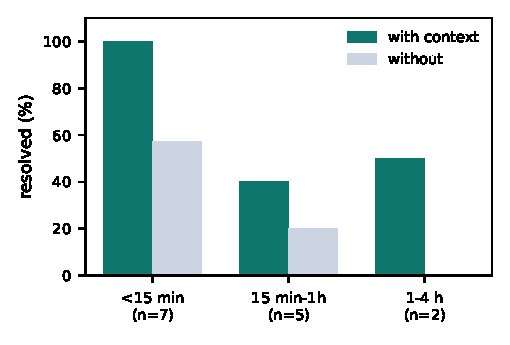
\includegraphics[width=0.55\linewidth]{figures/f2_swebench.pdf}
\caption{Resolved rate by dataset difficulty bucket, with and without context compilation.
Sample sizes are shown under each bucket; two baseline-red instances are excluded.
Data: Table~\ref{tab:difficulty} and the fact ledger.}
\label{fig:swebench}
\end{figure}

\begin{figure}[t]
\centering
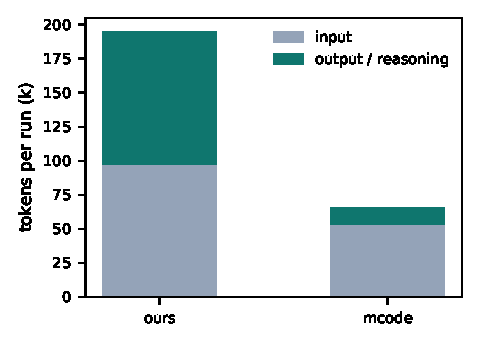
\includegraphics[width=0.55\linewidth]{figures/f3_cost.pdf}
\caption{Token composition per run for the two scaffolds on the same six tasks and model.
The gap is dominated by output (reasoning) tokens rather than by prompt size.
Data: the per-arm token accounting reported above.}
\label{fig:cost}
\end{figure}

% FACTS-USED: A1, A2, A3, A4, A5, A6, A7, A8, A9, A10, A11, A12, A13, B1, B2, B3, C1, C2, C3, C4, C5, C6, C7, D1, F1, F2, F3, F4, G1, G2, G4, H1, H2
